Temperature analysis of electronic systems is chiefly based on the duality
between the transfer of heat and the transfer of electric charge
\cite{kreith2000}. The core idea is to construct a so-called thermal \up{RC}
circuit for the system under consideration \cite{skadron2003}. Such a circuit is
a collection of thermal nodes that are characterized by thermal capacitances and
connected with each other via thermal resistances. The circuit is to capture the
relevant physical structure and thermal properties of the system and, thereby,
to model the system's thermal dynamics.

Consider now a generic electronic system that consists of \nc processing
elements and is equipped with a thermal package. The processing elements are the
active components of the system, that is, those that consume power. The thermal
package is the cooling equipment of the system including any passive components,
that is, those that do not consume power. Processing elements can be identified
at different levels of granularity; for instance, a processing element can be a
whole \up{SoC}, an individual \up{CPU}, or even an \up{ALU}. A thermal \up{RC}
circuit can also be constructed at different levels of granularity, which
primarily refers to the number thermal nodes, denoted by \nn in what follows,
and their placement. It should be understood that the chosen granularity has a
profound impact on the accuracy of the subsequent temperature analysis.

\begin{figure*}
  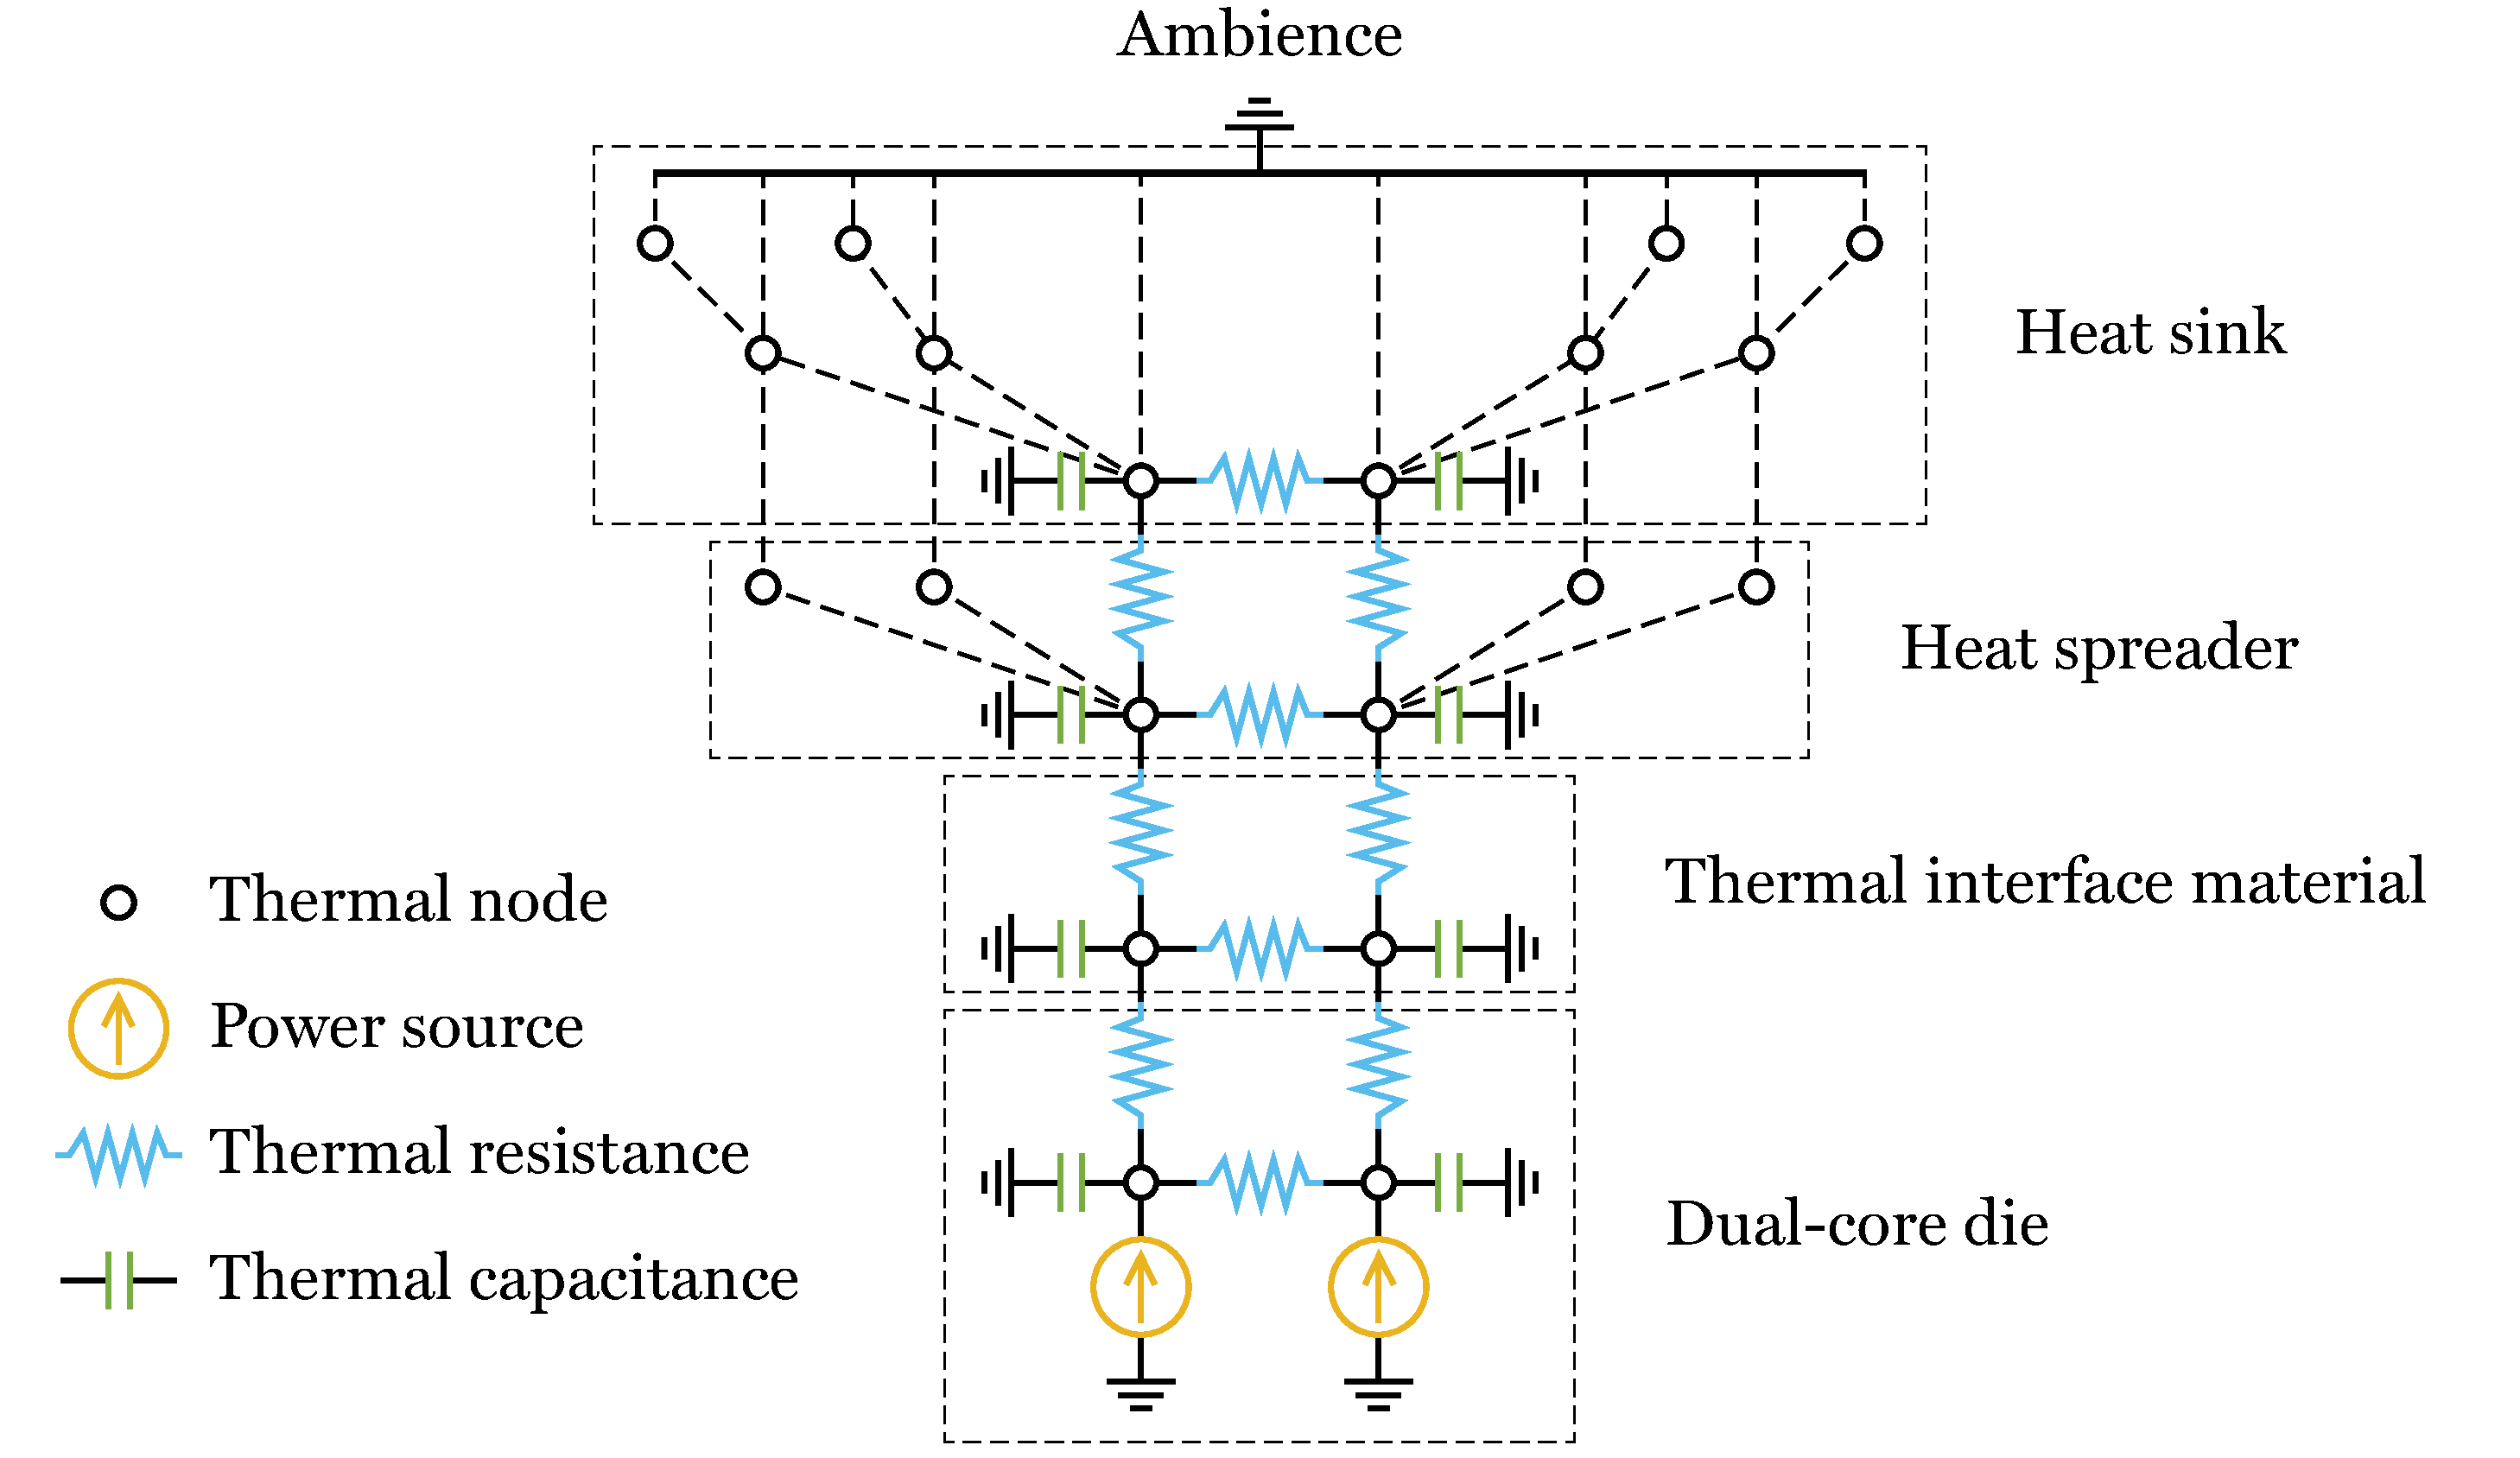
\includegraphics[width=1.0\textwidth]{include/assets/figures/circuit.pdf}
  \caption{Example of a thermal \up{RC} circuit.}
  \flab{circuit}
\end{figure*}

In order to give a better intuition about thermal \up{RC} circuits,
\fref{circuit} depicts a simplified example of a circuit constructed for a
hypothetical dual-core chip equipped with a thermal package composed of a
thermal interface material, heat spreader, and heat sink. Each of the $\nc$
processing elements is represented by one thermal node, and the thermal
interface material, heat spreader, and heat sink are captured by \nc, $\nc + 4$,
and $\nc + 8$ nodes, respectively. Thus, the total number of thermal nodes \nn
is $4 \times \nc + 12$. In this example, $\nc = 2$ and $\nn = 20$. The general
construction principle described above is the one presented in
\cite{skadron2003, huang2008}, and it is also the one used throughout this
thesis.

Suppose now that an adequate thermal \up{RC} circuit has been constructed for
the considered electronic system. Regardless of the structure of the circuit,
the thermal dynamics of the circuit (and the electronic system) are governed by
the following system of $\nn$ differential and $\nc$ algebraic equations:
\begin{subnumcases}{\elab{temperature-model-original}}
  \m{C} \frac{d\tvs(t)}{dt} + \m{G} \tvs(t) = \tm{B} \vp(t) \elab{temperature-differential-original} \\
  \vq(t) = \transpose{\tm{B}} \tvs(t) + \vq_\ambient \elab{temperature-algebraic-original}
\end{subnumcases}
In \eref{temperature-model-original}, $\vq \in \real^\nc$, $\vq_\ambient \in
\real^\nc$, and $\vp \in \real^\nc$ are vectors of the operating temperature,
ambient temperature, and power dissipation of the processing elements,
respectively. Further, $\tvs \in \real^\nn$ represents the state of the thermal
nodes, and $\m{C} \in \real^{\nn \times \nn}$ and $\m{G} \in \real^{\nn \times
\nn}$ are a diagonal matrix of the thermal capacitance and a symmetric and
positive-definite matrix of the thermal conductance, respectively. Lastly,
$\tm{B} \in \real^{\nn \times \nc}$ is a mapping between the processing elements
and the thermal nodes, which, without loss of generality, is assumed to be a
rectangular diagonal matrix whose diagonal elements are equal to unity.

It can be seen in \eref{temperature-model-original} that the input to
temperature analysis is power, and the output is temperature. For practical
computations, these quantities should be discrete. To this end, we introduce the
notions of a power and a temperature profile. A power profile of the system is
defined to be an $\nc \times \ns$ matrix
\[
  \mp = \left( \range{\vp_1}{\vp_\ns} \right)
  := \left( \range{\vp(t_1)}{\vp(t_\ns)} \right) \in \real^{\nc \times \ns}
\]
that contains \ns samples of the power consumption of the \nc processing
elements at \ns time moments with a certain sampling interval \dt. Similarly, a
temperature profile is defined to be an $\nc \times \ns$ matrix
\[
  \mq = \left( \range{\vq_1}{\vq_\ns} \right)
  := \left( \range{\vq(t_1)}{\vq(t_\ns)} \right) \in \real^{\nc \times \ns}
\]
that captures the heat dissipation of the processing elements over a number of
equidistant time moments. Even though the exact time frame and sampling interval
of a power or a temperature profile are not included in the above notation, they
are typically understood from the context.
